\chapter{Introduction} \label{ch:introduction}
 In a world full of constant uncertainties and disruptions, it is quintessential to have a sense of awareness and preparedness in order to avoid the losses or keep the losses as minimum as possible. The ability of a firm to withstand such uncertainties/disruptions and maintain the operational performance proves to have an advantage over the competitors. To comprehend the impact of these disruptions in the supply chains of firms, we need to have a fundamental understanding of several concepts first. These concepts include resilience, robustness, SC resilience and robustness, disruption propagation, network structure of the supply chain, and the implementation of simulation in supply chain design. The elaboration on these concepts is made in this chapter in the following sections.

\section{The Concept of Resilience and Robustness}
The fundamental idea of resilience has a foundation in almost all fields. In the article published by (\citeauthor{Boin2010}, \citeyear{Boin2010}) resilience can be observed in the fields such as engineering, biology, and psychiatry. Even though they have different meanings in their particular domains, the idea of resilience remains the same. Another definition as put by (\citeauthor{Westrum2006}, \citeyear{Westrum2006}) states that resilience is the ability prevent something bad from happening, ... to prevent something bad from becoming worse, or ... the ability to recover from something bad once it has happened.  (\citeauthor{HaleA.&Heijer2006}, \citeyear{HaleA.&Heijer2006}) define resilience as, ``...the ability in difficult conditions to stay within the safe envelope and avoid accidents". 

The resilience triangle is shown in Fig \ref{Resilience Triangle}. The quality of infrastructure percentage can be replaced by system performance to keep it as a generic measure. The main target over here is to keep the triangle as small as possible i.e the length between time $t_{\text{0}}$ and $t_{\text{1}}$ should be made as minimum as possible for a system to be highly resilient. There are many strategies that can be implemented to shorten the time length. The strategy that has been used in our study is a mix of contingency planning and key indicators identification. The implementation of these strategies is exhibited in the latter sections of our study.


Robustness has been defined by (\citeauthor{Tierney2007}, \citeyear{Tierney2007}) as ``the ability of systems, system elements,
and other units of analysis to withstand disaster
forces without significant degradation or loss of
performance". In simpler words, if the system is robust, then it should be able to continue its operations in the face of disruptions. The system does not exhibit robustness on its own. There are certain modifications that need to be occurred at the time of disruption at various levels by using methods of forecasting and planning. If these decisions are not taken at the intended time, then the system fails to obtain the state of robustness. 

\begin{figure}
  \centering
  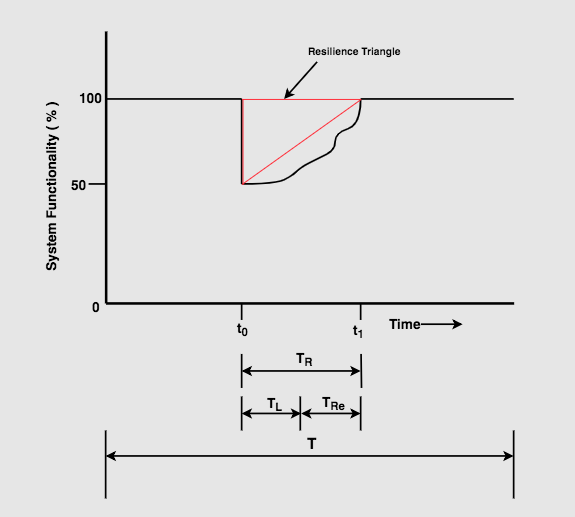
\includegraphics[width=6.5in]{figures/pdf/Resilience-Triangle.png}\\
  \caption{Resilience Triangle} \label{Resilience Triangle}
\end{figure}

\newpage
\section{Resilience and Robustness in Supply Chain}
Now that the understanding of the concepts of resilience and robustness has been established, let us incorporate these concepts into supply chain and find the significance they hold. The primary definitions for these concepts remain the same, but the supply chain is considered as our system in this case. (\citeauthor{Brandon-JonesE.;SquireB.;Autry2014},  \citeyear{Brandon-JonesE.;SquireB.;Autry2014})  have defined SC Resiliency as `` the ability of a system to return to its original state, within an acceptable period of time, after being disrupted". Resilience aids in indicating the weakest links of the chain and fortify them such that in the event of a similar disruption in the future, the system would be easily able to deal with it. (\citeauthor{Kitano2004}, \citeyear{Kitano2004}) defines SC Robustness as ``the ability of the supply chain to maintain its function despite internal or external disruptions".

These two concepts are coming into the light and  starting to have a pivotal role in the enhancement in the performance of the system due to rise in the number of uncertainties and unanticipated natural disasters. Incorporating these two factors into a supply chain would give the competitive advantage over others in the highly complex market.

SC resiliency and robustness ensures that there is a constant flow of materials and information throughout the supply chain. Even a hold up of materials in any facility within a SC of the firm makes a huge impact in terms of both time and money. Along with this, there are chances that the customer may decide to change to other firms due to the dissatisfaction caused to them. Various big companies such as Proctor and Gamble, Coca-Cola, Boeing, and Cisco have shifted their attention towards the implementation of resilience and robustness in their supply chains. 

\newpage
\section{Disruption Propagation}
Considerable research has been invested in understanding, predicting, preventing, and managing disruptions  (\citeauthor{Ivanov2016}, \citeyear{Ivanov2016}). The propagation of the disruption within a supply chain directly impacts the outcome. It is of utmost importance to focus on the supply chain disruption propagation because as the disruption spreads, the negative effects disseminate throughout the supply chain until the whole system fails. It is necessary to address the disruption at any level irrespective of its magnitude. A disruption which may seem innocuous has the potential to turn into a critical and harmful disruption by propagating and amplifying through various levels of the supply chain. The factors that affect the propagation of the supply chain disruption should be comprehended for better addressing of the disruptions.

The qualitative analysis made through the Gioia methodology mentioned by (\citeauthor{Scheibe2017}, \citeyear{Scheibe2017}) validates the data analysis to be done in three different orders. The first order analysis describes and summarizes the data. The second order analysis reduces the data by grouping similar codes and descriptions. The third order analysis consolidates the second-order themes into logical groupings called aggregate dimensions. There are three aggregate dimensions having two second-order themes each. These aggregate dimensions are 

1) Nature of the Disruption

2) Supply Chain Structure and Dependence 

3) Managerial Decision Making

The nature of the disruption itself affects the severity of the propagation of the disruption. The better understanding of the nature of the disruption poses as the foundation element in managing the disruption propagation. The two second-order themes associated with the nature of the disruption are correlation of risks and compounding effects. The correlation of risks theme states that one risk or even a risk mitigation strategy can inflict another risk. The disruptions never happen in a single member along a supply chain. Due to the strong interdependent and connected nature of the supply chain, disruptions never occur as an isolated event. The compounding effect means the adhering of one disruption to other as it propagates along the supply chain. Due to the compounding effect, the disruptions grow in size and severity. The decision-making capability of the stakeholders directly contributes to the compounding effect. Self-preservation or measures to mitigate the risk at a personal level increases the severity of the disruption. The structure of the supply chain and the consisting dependencies serve as a source of propagation of disruption along the supply chain.

The two second-ordered themes associated with the supply chain structure and dependence are cyclical linkages and counterparty risk as shown in Fig \ref{Aggregate Dimensions}. The cyclical linkages are nothing but the inter-dependencies between the nodes of a supply chain. A problem in one node leads to a problem in another node and vice versa. These linkages often go unnoticed until the disruptions occur. The cyclical linkages occur as a reason of one or more members playing different roles at different levels in the same supply chain. To mitigate the supply chain disruption propagation, the cyclical linkages must be carefully observed and studied. Counterparty risk occurs when one supplier supplies to a firm and its competitor at the same time. This means that the risk in one link in the supply chain is dependent on the other link. It is arduous to identify the interconnection through which the disruption can propagate. The firm focuses on one interconnection within a supply chain when the risk through different parts of the supply chain hit the firm without having any knowledge of it. The counterparty risk takes place mainly due to the hiding of information within the supply chain members (\citeauthor{Scheibe2017}, \citeyear{Scheibe2017}). 

The managerial decision-making at the time of disruptions also affect the propagation through the supply chain. The two-second ordered themes associated with this type of aggregate dimension are herding behavior and misaligned incentives as shown in Fig \ref{Aggregate Dimensions} (\citeauthor{Scheibe2017}, \citeyear{Scheibe2017}). The herding behavior is the behavior in which one person behaves the way that others behave even though they are completely different people. In case of a supply chain, during the time of disruption, a firm takes the same measures as others are taking to mitigate the disruption although they have different properties and structure. They just tend to follow the 'herd' without thinking. The easiest example of herding behavior is when food joints adjust their prices based on other food joints which are the competitors. Misaligned incentives are the decisions made by the supply chain decision-makers which benefits one part of the supply chain at the expense of the other parts in the supply chain. These decisions are a result of the inability of the decision-makers to see the bigger picture and improve the entire supply chain rather than improving just one part of it. One such misaligned incentive is giving more importance to taking actions after a disruption takes place rather than taking actions to avoid the disruption from happening. 


\begin{figure}[H]
  \centering
  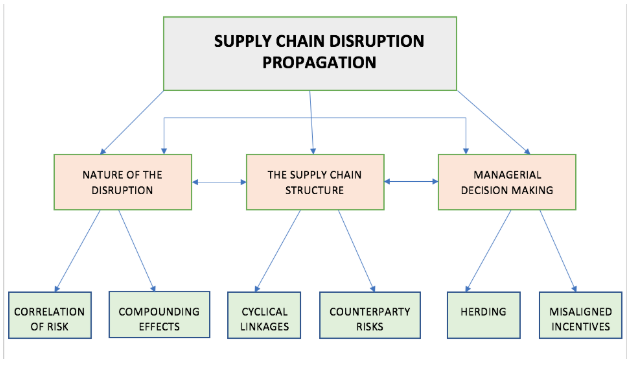
\includegraphics[width=4.5in]{figures/pdf/Aggregate-Dimensions.png}\\
  \caption{Aggregate Dimensions and their Second-order themes.}\label{Aggregate Dimensions}
\end{figure}

In a supply chain, the aggregate dimensions are the major source of the disruption propagation. If the risks in these aggregate dimensions are mitigated and the supply chain is designed in such a way that it would avoid any disruption propagation, then the resiliency of the supply chain is increased. There has been ample research related to the identification of the risks associated with the aggregate dimensions but there has not been a lot of research in the field of mitigation of the disruption propagation through the aggregate dimensions (\citeauthor{Scheibe2017}, \citeyear{Scheibe2017}). The nature of disruption, supply chain structure, and managerial decisions are the aggregate dimensions through which the supply chain disruption propagation can be contained.

The Figure \ref{Aggregate Dimensions} represents the aggregate dimensions on which the supply chain disruption propagation is dependent on. It also shows the second order themes which contribute to the aggregate dimensions. Out of these, correlation of risk and cyclical linkages have a significant impact on the disruption propagation. Hence, the main focus of this paper would be to model a supply chain in such a manner that the problems arising in the supply chain due to these factors could be anticipated and mitigated at the initial stages to avoid cascading of the failure through the supply chain.

\subsection{Correlation of Risks}
The supply chain is a network of strongly interconnected nodes which function together in coordination for getting the desired output. If there is a disruption occurring at any level in the supply chain, it is plausible to affect the performance of the supply chain. It is observed that this disruption does not just affect the point of occurrence, but it may be propagated throughout the SC because of the inter-connectivity. The disruption may travel upstream as well as downstream the SC. This phenomenon is called as the ripple effect in the supply chain (\citeauthor{ivanov2017simulation}, \citeyear{ivanov2017simulation}). It is highly unlikely for a disruption to occur in isolation. It is not just the risk that can cause another risk, but the strategy to mitigate one risk can also lead to risk in a different node in the SC. Thus, the risk mitigation strategy should not be focused only on reducing the risk at a certain point, but it should also pay close attention towards the effects of the risk as well as the effects of the mitigation technique on other elements of the SC.

The Figure \ref{Ripple effect} represents the ripple effect in a supply chain structure. It can be evidently seen that the disruption is going to propagate in both directions. It is important to minimize the risk caused due to the disruption. At the same time, the risks associated with the mitigation strategy should also be taken into consideration. The decisions that are taken once the disruption occurs play a vital role in the degree of recovery of the SC. The managerial decisions during disruption about these decision variables and the ripple effect analysis throughout the SC will contribute towards the resilience of the SC.

The methodology that has been suggested for limiting the propagation of risks due to the correlation of risks is the ripple effect modeling. With the help of this methodology, the effect of the disruption and the effect of the strategies devised to reduce the risks due to the disruption can be found out throughout the supply chain structure. This will help in making the supply chain more resilient by reducing the risks after the disruption has occurred.

\begin{figure}[H]
  \centering
  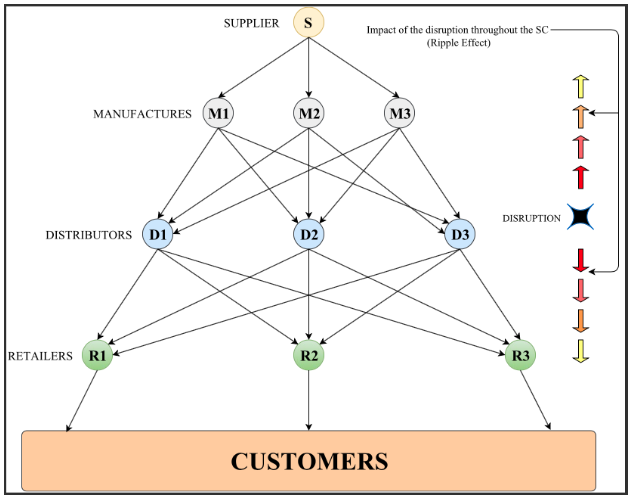
\includegraphics[width=6.5in]{figures/pdf/Ripple-effect.png}\\
  \caption{Ripple effect in the Supply Chain Structure.}\label{Ripple effect}
\end{figure}

\newpage
\subsection{Cyclical Linkages}

In a supply chain, all the nodes are inter-connected and are inter-dependent. This aids in the desired functioning of the supply chain. At the same time, if there is any disruption in the SC, the same inter-connectivity and inter-dependence will become disadvantageous. Suppose that there are three nodes in a supply chain. If there is a problem in node 1, then it can transmit a problem to node 2. Similarly, if there is a problem in node 2, it may propagate to node 3. The problem in node 3 can have a feedback effect on the first node. This is called as the cyclical linkage in supply chain and is shown in Fig \ref{Cyclical Linkage}. A disruption in one of the stages of trade-off can lead to a disruption in the other stages due to the cyclical linkage. Thus affecting the entire supply chain at different levels.

\begin{figure}[H]
  \centering
  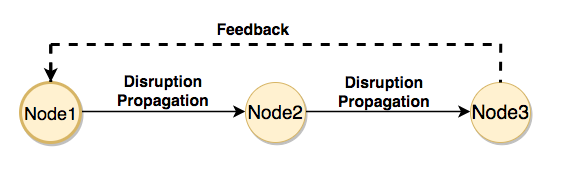
\includegraphics[width=4.0in]{figures/pdf/Cyclical-Linkage.png}\\
  \caption{Cyclical Linkage Representation}\label{Cyclical Linkage}
\end{figure}


The disruptions occurring in the cyclical linkages are the most underestimated in the entire supply chain. But, these have a very significant impact on the supply chain. These linkages should be considered from all the perspectives. There exists different cyclical linkages between different levels of the supply chain. There is a customer order cycle between the customer and the retailer; a replenishment cycle between the retailer and the distributor; a manufacturing cycle between distributor and the manufacturer; a procurement cycle between the manufacturer and the supplier. Any disruption in one of these cycles can lead to the disruption of the whole supply chain. 

The customer order cycle consists of 4 distinctive activities. These are customer arrival, customer order entry, customer order fulfillment, and customer order receiving. The replenishment cycle consists of retail order trigger, retail order entry, retail order fulfillment, and retail order receiving. The manufacturing cycle consists of order arrival, production scheduling, manufacturing and shipping, and receiving. The procurement cycle consists of order based on manufacturer's production schedule or supplier's stocking method, supplier production scheduling, component manufacturing and shipping, and receiving at manufacturer.



\newpage
\section{Network Structure}

(\citeauthor{Kim2015}, \citeyear{Kim2015}) have considered the network structural perspective for the supply network disruption and resilience. It can be inferred that in a network, the prime cause of interruption of the movement of the unit is the malfunction in the node or arc. Although it is the prime reason for the cause of interruption, it does not help in detecting the network-level disruption. In this paper, the methodology that has been used for the purpose of designing the supply chain network is the graph theory. It has been applied to a great extent to the complex networks like the World Wide Web, power grids, and the food chains (\citeauthor{gross2005graph}, \citeyear{gross2005graph}). If we implement the graph theory in the field of supply chain, then the facilities would be a representation of the nodes, whereas, the logistics between the facilities would be represented by the arcs.

\begin{figure}[H]
  \centering
  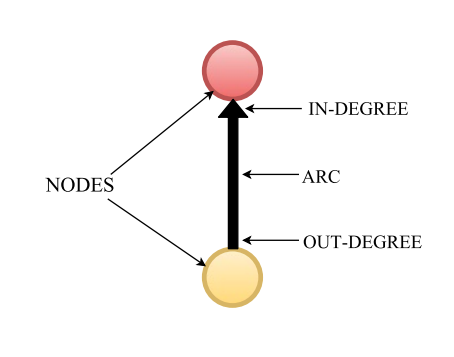
\includegraphics[width=2.5in]{figures/pdf/Node-structure.png}\\
  \caption{The structure of nodes and arcs according to the graph theory.}\label{Node structure}
\end{figure}


The latent structure of a supply chain network can be explained by the graph theory in a suitable manner. Instead of using the notations G = (V, E) (\citeauthor{emden1997complexity}, \citeyear{emden1997complexity}) ,the notation G=(N, A) is used in terms of supply chain design (\citeauthor{Kim2015}, \citeyear{Kim2015}). The set N contains the nodes while the set A contains the arcs of the supply chain network. It glances at the correlation between the nodes and arcs at a structural level from a meticulous perspective. The in-degree and out-degree are the elements that describe the amount of the supplier and customer present in the node in consideration. The in-degree resembles the number of arcs whose head connects to a node, and the out-degree resembles the number of arcs whose tail connects to the node. 

In the event of an arc or node level disruption, it has been observed that the supply chain may still continue to function normally, as there exists multiple walks from the initial node to the final node. The disruption does not seem to be affecting the supply chain network, since the materials are being delivered to their required final point from its initial point. But, the network level disruption can cause the system to fail or the process to remain incomplete.

For determining the performance of the network structure, a theoretical framework is provided by the complex adaptive systems (CAS) theory (\citeauthor{Kim2015}, \citeyear{Kim2015}). According to this theory, the analytic frameworks have been developed for the better understanding of the correlations between all the elements within the system. It sheds light on how these correlations affect the overall performance of the system. The structures that have been taken into consideration in this research paper are the ones that take place in the real-life SC scenario. These are as following:


\begin{itemize}
    \item Block-diagonal network structures
    \item Scale-free network structures
    \item Centralized network structures
    \item Diagonal network structures
\end{itemize}

The block-diagonal network structure is the one in which the nodes are clumped up between the initial and final node, where there are connections within the clumps but not between the clumps. The scale-free network pattern exhibits a biased nature, where a certain few nodes have most of the connections, while most of the other nodes obtain the merest of connections. This type of network pattern has node degree distribution which is highly distorted and seems to follow a power-law or Pareto distribution. The centralized structure is an accurate illustration of highly central nodes. In this, the high-level suppliers assume authority as a representative of the customer firm in the design and development processes. The diagonal supply structure follows a certain pecking order in which the materials are moved only in one direction (from the lower-level nodes to the higher-level node). These network structures are as shown Fig \ref{BDNS}, Fig \ref{SFNS}, Fig \ref{CNS}, and Fig \ref{DNS}.

\begin{figure}[H]
  \centering
  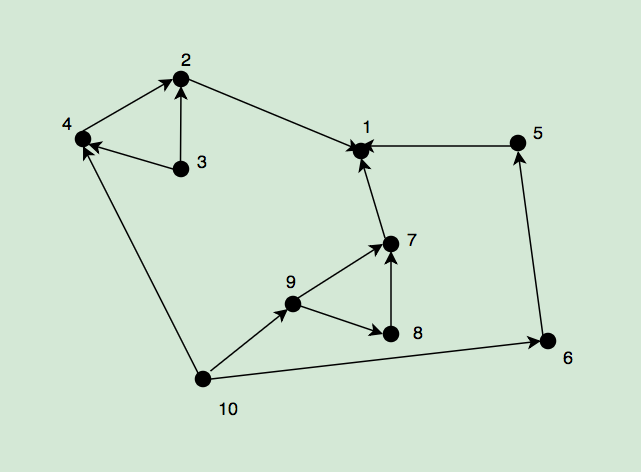
\includegraphics[width=4.5in]{figures/pdf/Block-diagonal.png}\\
  \caption{Block-Diagonal Network Structure} \label{BDNS}
\end{figure}

\begin{figure}[H]
  \centering
  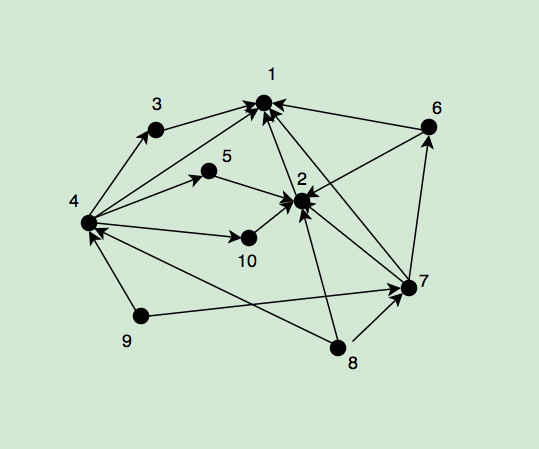
\includegraphics[width=4.5in]{figures/pdf/ScaleFree.png}\\
  \caption{Scale-free Network Structure} \label{SFNS}
\end{figure}

\begin{figure}[H]
  \centering
  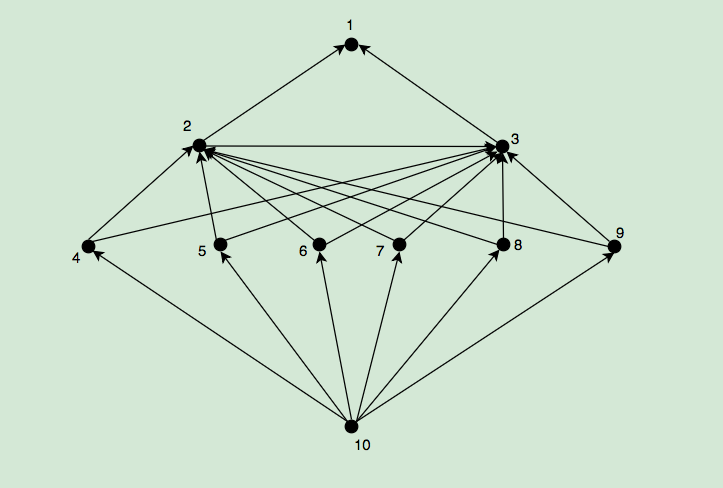
\includegraphics[width=4.5in]{figures/pdf/Centralized.png}\\
  \caption{Centralized Network Structure} \label{CNS}
\end{figure}

\begin{figure}[H]
  \centering
  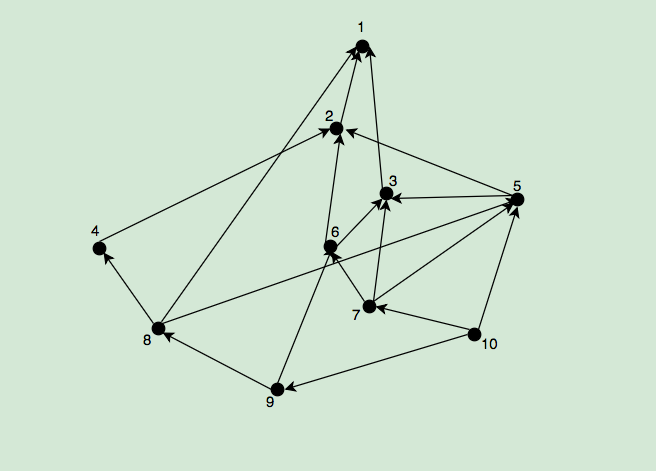
\includegraphics[width=4.5in]{figures/pdf/Diagonal.png}\\
  \caption{Diagonal Network Structure} \label{DNS}
\end{figure}

\newpage
For the evaluation of the best network structure, certain metrics are required to be defined and measured for all the structures. Based on these metrics, the resiliency of the structure can be determined. In this paper, the authors have defined and measured some resilience metrics that would be helpful in determining the resiliency of the network structures in consideration.

These resilience metrics are as follows:


\textbf{Network Density ($N_{\text{D}}$) :}
\begin{equation}
    N_D = \frac{N_T}{N_P}
\end{equation}
\newline
Where,
\newline
  $N_{\text{T}}$ = No. of total existing arcs
\newline  
 $N_{\text{P}}$ = No. of possible arcs
 

\textbf{Average In-Degree:} It is the mean of the number of arcs having their heads connected to the nodes throughout the network.

\textbf{Average Out-Degree:} It is the mean of the number of arcs having their tails connected to the nodes throughout the network.

\textbf{Connectivity:} It is the minimum number of nodes and/or arcs which when removed will disengage the network.

A supply network disruption occurs when the network is incomplete between the initial and final node due to the disruptions in the nodes/arcs. The supply network resilience can be determined by evaluating the probability that in case of a removal of a random node/arc between the nodes, then the network is still being completed between the initial and the final node.


Thus, the supply network resilience ($R_{\text{S}}$) can be written down mathematically as
\begin{equation}
   R_S = \frac{N_U}{N_D}
\end{equation}
Where,
\newline
$N_{\text{U}}$ = Total no. of node/arc disruptions, which do not lead to disruption
\newline
$N_{\text{D}}$ = Total no. of node/arc disruptions

On calculating and comparing these metrics for the structures that have been considered for the study, it is observed that the scale-free network structure has the highest score on the resilience index. It can be inferred from the calculations that the higher resilience does not necessarily come from the networks that are closely-packed or intricate. From the viewpoint of the network structures, a plethora of network does not yield an increase in resilience. In case of unanticipated disruptions, the network that has various tiers has a better chance of survival. The manner in which the nodes and arcs are connected to each other in a network influences the disruption risk and its resilience against the disruption.

Thus, from the aforementioned research it can be extrapolated that the network structure has a significant impact on the resiliency of the entire system. The resiliency of the supply chain network is impacted by the number of nodes and arcs it is made up of. The metrics such as network density, average in-degree, average out-degree, connectivity, and resilience can be further applied to the concepts of cyclical linkages and the correlation of risks in the supply chain. Thus, these two concepts can be further worked on for aiding the improvement of the resilience of the supply chain.


\section{Implementation of Simulation in Supply Chain Design} 
    
In today's world the nature of the supply chain has become very complex both in size and structure. There are multiple players and facilities present in them. Due to inter-connectivity and inter-dependencies present in them, the supply chains are prone to have disruptions that may disseminate throughout the network. If the supply chains are relatively small, then the uncertainties can be easily mitigated through the techniques of communication and managerial decisions due to the involvement of few players. On the other hand, if the supply chain is considerably large, then the same techniques would prove to be useless. A lot of significant information would be lost somewhere along the communication. Thus, there arises a need for using simulation software that provide an environment to model supply chains having any number of players and facilities and in real time. It is possible to model the supply chain at individual levels so that each player can be considered very carefully. This aids us in making modifications in the parameters at the individual level in the face of disruption, such that there is a sense of continuity maintained throughout the supply chain. Thus, making the supply chain resilient and robust. The simulation software helps us in quantifying our methodology. Alternate facility selection can be easily achieved through the simulation software. The facilities are selected in such a manner that they can fulfill the needs of the disrupted facility in less time and less cost. Simulation allows us the flexibility to work with different alternatives to resolve the impact of disruptions on the supply chain. It also helps us in understanding the ripple effect of disruptions and its impact throughout the supply chain.



